\documentclass[journal]{IEEEtran}

\usepackage{cite}

% *** GRAPHICS RELATED PACKAGES ***
%
\ifCLASSINFOpdf
  % \usepackage[pdftex]{graphicx}
  % declare the path(s) where your graphic files are
  % \graphicspath{{../pdf/}{../jpeg/}}
  % and their extensions so you won't have to specify these with
  % every instance of \includegraphics
  % \DeclareGraphicsExtensions{.pdf,.jpeg,.png}
\else
  % or other class option (dvipsone, dvipdf, if not using dvips). graphicx
  % will default to the driver specified in the system graphics.cfg if no
  % driver is specified.
  % \usepackage[dvips]{graphicx}
  % declare the path(s) where your graphic files are
  % \graphicspath{{../eps/}}
  % and their extensions so you won't have to specify these with
  % every instance of \includegraphics
  % \DeclareGraphicsExtensions{.eps}
\fi
% graphicx was written by David Carlisle and Sebastian Rahtz. It is
% required if you want graphics, photos, etc. graphicx.sty is already
% installed on most LaTeX systems. The latest version and documentation
% can be obtained at: 
% http://www.ctan.org/pkg/graphicx
% Another good source of documentation is "Using Imported Graphics in
% LaTeX2e" by Keith Reckdahl which can be found at:
% http://www.ctan.org/pkg/epslatex
%
% latex, and pdflatex in dvi mode, support graphics in encapsulated
% postscript (.eps) format. pdflatex in pdf mode supports graphics
% in .pdf, .jpeg, .png and .mps (metapost) formats. Users should ensure
% that all non-photo figures use a vector format (.eps, .pdf, .mps) and
% not a bitmapped formats (.jpeg, .png). The IEEE frowns on bitmapped formats
% which can result in "jaggedy"/blurry rendering of lines and letters as
% well as large increases in file sizes.
%
% You can find documentation about the pdfTeX application at:
% http://www.tug.org/applications/pdftex





% *** MATH PACKAGES ***
%
\usepackage{amsmath}
% A popular package from the American Mathematical Society that provides
% many useful and powerful commands for dealing with mathematics.
%
% Note that the amsmath package sets \interdisplaylinepenalty to 10000
% thus preventing page breaks from occurring within multiline equations. Use:
%\interdisplaylinepenalty=2500
% after loading amsmath to restore such page breaks as IEEEtran.cls normally
% does. amsmath.sty is already installed on most LaTeX systems. The latest
% version and documentation can be obtained at:
% http://www.ctan.org/pkg/amsmath





% *** SPECIALIZED LIST PACKAGES ***
%
\usepackage{algorithmic}
% algorithmic.sty was written by Peter Williams and Rogerio Brito.
% This package provides an algorithmic environment fo describing algorithms.
% You can use the algorithmic environment in-text or within a figure
% environment to provide for a floating algorithm. Do NOT use the algorithm
% floating environment provided by algorithm.sty (by the same authors) or
% algorithm2e.sty (by Christophe Fiorio) as the IEEE does not use dedicated
% algorithm float types and packages that provide these will not provide
% correct IEEE style captions. The latest version and documentation of
% algorithmic.sty can be obtained at:
% http://www.ctan.org/pkg/algorithms
% Also of interest may be the (relatively newer and more customizable)
% algorithmicx.sty package by Szasz Janos:
% http://www.ctan.org/pkg/algorithmicx




% *** ALIGNMENT PACKAGES ***
%
\usepackage{array}
% Frank Mittelbach's and David Carlisle's array.sty patches and improves
% the standard LaTeX2e array and tabular environments to provide better
% appearance and additional user controls. As the default LaTeX2e table
% generation code is lacking to the point of almost being broken with
% respect to the quality of the end results, all users are strongly
% advised to use an enhanced (at the very least that provided by array.sty)
% set of table tools. array.sty is already installed on most systems. The
% latest version and documentation can be obtained at:
% http://www.ctan.org/pkg/array


% IEEEtran contains the IEEEeqnarray family of commands that can be used to
% generate multiline equations as well as matrices, tables, etc., of high
% quality.




% *** SUBFIGURE PACKAGES ***
%\ifCLASSOPTIONcompsoc
%  \usepackage[caption=false,font=normalsize,labelfont=sf,textfont=sf]{subfig}
%\else
%  \usepackage[caption=false,font=footnotesize]{subfig}
%\fi
% subfig.sty, written by Steven Douglas Cochran, is the modern replacement
% for subfigure.sty, the latter of which is no longer maintained and is
% incompatible with some LaTeX packages including fixltx2e. However,
% subfig.sty requires and automatically loads Axel Sommerfeldt's caption.sty
% which will override IEEEtran.cls' handling of captions and this will result
% in non-IEEE style figure/table captions. To prevent this problem, be sure
% and invoke subfig.sty's "caption=false" package option (available since
% subfig.sty version 1.3, 2005/06/28) as this is will preserve IEEEtran.cls
% handling of captions.
% Note that the Computer Society format requires a larger sans serif font
% than the serif footnote size font used in traditional IEEE formatting
% and thus the need to invoke different subfig.sty package options depending
% on whether compsoc mode has been enabled.
%
% The latest version and documentation of subfig.sty can be obtained at:
% http://www.ctan.org/pkg/subfig




% *** FLOAT PACKAGES ***
%
% \usepackage{fixltx2e}
% fixltx2e, the successor to the earlier fix2col.sty, was written by
% Frank Mittelbach and David Carlisle. This package corrects a few problems
% in the LaTeX2e kernel, the most notable of which is that in current
% LaTeX2e releases, the ordering of single and double column floats is not
% guaranteed to be preserved. Thus, an unpatched LaTeX2e can allow a
% single column figure to be placed prior to an earlier double column
% figure.
% Be aware that LaTeX2e kernels dated 2015 and later have fixltx2e.sty's
% corrections already built into the system in which case a warning will
% be issued if an attempt is made to load fixltx2e.sty as it is no longer
% needed.
% The latest version and documentation can be found at:
% http://www.ctan.org/pkg/fixltx2e


% \usepackage{stfloats}
% stfloats.sty was written by Sigitas Tolusis. This package gives LaTeX2e
% the ability to do double column floats at the bottom of the page as well
% as the top. (e.g., "\begin{figure*}[!b]" is not normally possible in
% LaTeX2e). It also provides a command:
%\fnbelowfloat
% to enable the placement of footnotes below bottom floats (the standard
% LaTeX2e kernel puts them above bottom floats). This is an invasive package
% which rewrites many portions of the LaTeX2e float routines. It may not work
% with other packages that modify the LaTeX2e float routines. The latest
% version and documentation can be obtained at:
% http://www.ctan.org/pkg/stfloats
% Do not use the stfloats baselinefloat ability as the IEEE does not allow
% \baselineskip to stretch. Authors submitting work to the IEEE should note
% that the IEEE rarely uses double column equations and that authors should try
% to avoid such use. Do not be tempted to use the cuted.sty or midfloat.sty
% packages (also by Sigitas Tolusis) as the IEEE does not format its papers in
% such ways.
% Do not attempt to use stfloats with fixltx2e as they are incompatible.
% Instead, use Morten Hogholm'a dblfloatfix which combines the features
% of both fixltx2e and stfloats:
%
% \usepackage{dblfloatfix}
% The latest version can be found at:
% http://www.ctan.org/pkg/dblfloatfix




%\ifCLASSOPTIONcaptionsoff
%  \usepackage[nomarkers]{endfloat}
% \let\MYoriglatexcaption\caption
% \renewcommand{\caption}[2][\relax]{\MYoriglatexcaption[#2]{#2}}
%\fi
% endfloat.sty was written by James Darrell McCauley, Jeff Goldberg and 
% Axel Sommerfeldt. This package may be useful when used in conjunction with 
% IEEEtran.cls'  captionsoff option. Some IEEE journals/societies require that
% submissions have lists of figures/tables at the end of the paper and that
% figures/tables without any captions are placed on a page by themselves at
% the end of the document. If needed, the draftcls IEEEtran class option or
% \CLASSINPUTbaselinestretch interface can be used to increase the line
% spacing as well. Be sure and use the nomarkers option of endfloat to
% prevent endfloat from "marking" where the figures would have been placed
% in the text. The two hack lines of code above are a slight modification of
% that suggested by in the endfloat docs (section 8.4.1) to ensure that
% the full captions always appear in the list of figures/tables - even if
% the user used the short optional argument of \caption[]{}.
% IEEE papers do not typically make use of \caption[]'s optional argument,
% so this should not be an issue. A similar trick can be used to disable
% captions of packages such as subfig.sty that lack options to turn off
% the subcaptions:
% For subfig.sty:
% \let\MYorigsubfloat\subfloat
% \renewcommand{\subfloat}[2][\relax]{\MYorigsubfloat[]{#2}}
% However, the above trick will not work if both optional arguments of
% the \subfloat command are used. Furthermore, there needs to be a
% description of each subfigure *somewhere* and endfloat does not add
% subfigure captions to its list of figures. Thus, the best approach is to
% avoid the use of subfigure captions (many IEEE journals avoid them anyway)
% and instead reference/explain all the subfigures within the main caption.
% The latest version of endfloat.sty and its documentation can obtained at:
% http://www.ctan.org/pkg/endfloat
%
% The IEEEtran \ifCLASSOPTIONcaptionsoff conditional can also be used
% later in the document, say, to conditionally put the References on a 
% page by themselves.




% *** PDF, URL AND HYPERLINK PACKAGES ***
%
\usepackage{url}
% url.sty was written by Donald Arseneau. It provides better support for
% handling and breaking URLs. url.sty is already installed on most LaTeX
% systems. The latest version and documentation can be obtained at:
% http://www.ctan.org/pkg/url
% Basically, \url{my_url_here}.




% *** Do not adjust lengths that control margins, column widths, etc. ***
% *** Do not use packages that alter fonts (such as pslatex).         ***
% There should be no need to do such things with IEEEtran.cls V1.6 and later.
% (Unless specifically asked to do so by the journal or conference you plan
% to submit to, of course. )


% correct bad hyphenation here
\hyphenation{op-tical net-works semi-conduc-tor}


\begin{document}
%
% paper title
% Titles are generally capitalized except for words such as a, an, and, as,
% at, but, by, for, in, nor, of, on, or, the, to and up, which are usually
% not capitalized unless they are the first or last word of the title.
% Linebreaks \\ can be used within to get better formatting as desired.
% Do not put math or special symbols in the title.
\title{Battery Hardware Emulator\\ Module Design Document}
%
%
% author names and IEEE memberships
% note positions of commas and nonbreaking spaces ( ~ ) LaTeX will not break
% a structure at a ~ so this keeps an author's name from being broken across
% two lines.
% use \thanks{} to gain access to the first footnote area
% a separate \thanks must be used for each paragraph as LaTeX2e's \thanks
% was not built to handle multiple paragraphs
%

\author{Youri~Tils,
        Nikola~Panchev, 
        Robin~van~den~Dungen,
        Hein~Verhallen,
        Wyatt~Southard
% \thanks{M. Shell was with the Department
% of Electrical and Computer Engineering, Georgia Institute of Technology, Atlanta,
% GA, 30332 USA e-mail: (see http://www.michaelshell.org/contact.html).}% <-this % stops a space
% \thanks{J. Doe and J. Doe are with Anonymous University.}% <-this % stops a space
% \thanks{Manuscript received April 19, 2005; revised August 26, 2015.}
}

% The paper headers
\markboth{Fontys University of Applied Sciences, Eindhoven, 13/12/2023}%
{Shell \MakeLowercase{\textit{et al.}}: Battery Hardware Emulator Module Design Document}
% The only time the second header will appear is for the odd numbered pages
% after the title page when using the twoside option.
% 
% *** Note that you probably will NOT want to include the author's ***
% *** name in the headers of peer review papers.                   ***
% You can use \ifCLASSOPTIONpeerreview for conditional compilation here if
% you desire.




% If you want to put a publisher's ID mark on the page you can do it like
% this:
%\IEEEpubid{0000--0000/00\$00.00~\copyright~2015 IEEE}
% Remember, if you use this you must call \IEEEpubidadjcol in the second
% column for its text to clear the IEEEpubid mark.



% use for special paper notices
%\IEEEspecialpapernotice{(Invited Paper)}




% make the title area
\maketitle

% As a general rule, do not put math, special symbols or citations
% in the abstract or keywords.
\begin{abstract}
Abstract goes here.
\end{abstract}

% Note that keywords are not normally used for peerreview papers.
\begin{IEEEkeywords}
BatteryNL, BMS, Li-ion.
\end{IEEEkeywords}






% For peer review papers, you can put extra information on the cover
% page as needed:
% \ifCLASSOPTIONpeerreview
% \begin{center} \bfseries EDICS Category: 3-BBND \end{center}
% \fi
%
% For peerreview papers, this IEEEtran command inserts a page break and
% creates the second title. It will be ignored for other modes.
\IEEEpeerreviewmaketitle



\section{Background \& Introduction}
\IEEEPARstart
{E}{nergy} storage is one of the grand technological challenges posed by the transformation from a
fossil fuel dependent society to one that relies on renewable energy sources. Batteries provide
some good solutions to these challenges, however, the present battery technologies suffer from
high weight, short lifetime, long charging time and limited safety.

The BatteryNL consortium is focused on developing the next generation of more efficient
batteries with enhanced performance. Fontys Engineering is helping BatteryNL with the development 
of an optimized battery management system (BMS), testing which can be quite
hazardous. Modern batteries can store a lot of energy, and if they catch fire, can be difficult to
extinguish. In addition to that, an insufficiently tested BMS can pose a hazard to users and to
the environment.

The solution to that is to emulate the battery and the load, so that testing can be completed
under a wide range of conditions without taking excessive risks.

This document explains in detail the development process of this project. 
Architecture, hardware, software, testing and results are covered for every design 
iteration of the process. 

The design is based on the 14-cell slider battery pack emulator kit by 
NXP \cite{UM11349}.

\section{Project Description}
\IEEEPARstart
{T}{he} goal of this project is to design, build and test a battery pack emulator and (optionally)
a load emulator. The positive outcome of this development ensures a safe way of testing BMSs


The first iteration of the design include a Li-ion battery cell emulator, capable of charging and discharging small currents (100 mA) and
the voltage of the emulated cell is adjusted by a mechanical variable resistor. This iteration has no software and it is needed only for 
testing the current sourcing and sinking. This design is completed on a single PCB.

The second design iteration is made modular - consisting of a model board PCB and cell PCBS, and software is implemented to control the 
voltages of each emulated cell. The model board PCB has the microprocessor and is able to connect to and control up to 14 cell PCBs. Each
cell PCB includes all the circuitry needed to source and sink current up to 12 A, control the voltage and emulate the temperature via software.
Each emulated cell has a voltage and current range that is 20\% larger than the safe operating area of a Li-ion cell.



% Because the project team members are not yet experts in the field of designing battery pack
% emulators for BMS testing, it is chosen to design the battery pack emulator in iterations. In
% the first design iteration a battery pack emulator circuit will be designed which emulates the
% characteristics of a Li-ion battery pack. This battery pack emulator consists of two Li-ion cell
% emulators which are capable of charging and discharging. The voltages of each emulated cell are
% adjusted by a mechanical variable resistor. Each emulated cell has a voltage and current range
% that is 20\% larger than the safe operating area of a Li-ion cell.

% In the second design iteration software will be added to the battery emulator circuit to
% control the voltages of each emulated cell via software. Also the temperature will be emulated
% in the battery pack emulator. The third design iteration consists of expanding the amount of
% emulated cells in the emulated battery pack to 14 cells. In the fourth design iteration a load
% emulator will be designed to test the BMS under different load conditions. This load emulator
% is capable of emulating electronics and motors.

% At the end of the project it is expected that a battery pack emulator and optionally a load
% emulator is delivered. And if the planning allows it, a research report on existing battery and
% load emulators and the requirements for future battery and load emulators is delivered.
% % \hfill mds
 
% \hfill August 26, 2015

% \subsection{Subsection Heading Here}
% Subsection text here.

% % needed in second column of first page if using \IEEEpubid
% %\IEEEpubidadjcol

% \subsubsection{Subsubsection Heading Here}
% Subsubsection text here.

\section{Boundary Conditions}
\IEEEPARstart
{T}{he} project boundaries defines what falls out of the scope of the project. The following
things fall beyond the scope of this project:
\begin{itemize}
    \item Battery management system (BMS) research, This project will not research on how a BMS
    functions apart from the in and outputs a BMS typically has.
    \item BMS design, The project will not design or in any way or form create a BMS.
    \item User Interface(UI), The project will not include a UI to control the Hardware. 
    The hardware emulator will be controlled by adjusting the firmware.
    \item The research paper will only focus on our design work and future 
    specifications of a battery emulator.
\end{itemize}


\section{Project Approach}

\section{Requirements}
\IEEEPARstart
{F}{or} this project, the following non-functional requirements with their 
functional requirements have been specified. These requirements are set 
to ensure a successful iterative process, however, through the duration 
of the project some of them were changed. All the changes are explained
in the corresponding sections. The requirements go as follows:

\subsection{Non-functional requirements}
\begin{enumerate}
    \item[1.] Battery Pack emulator is able to emulate Li-ion characteristics.
    \item[2.] Battery pack emulator consists of two emulated Li-ion 
    cells(1st iteration).
    \item[3.] Battery pack emulator is able to emulate charging and discharging of
    Li-ion cells.
    \item[4.] The voltages of each emulated cell can be adjusted separately 
    via hardware (1st iteration).
    \item[5.] Each emulated cell has a voltage and current range that is 20\%
    larger than the safe operating area of a Li-ion cell.
    \item[6.] The voltages of each emulated cell can be adjusted separately 
    via software (2nd iteration).
    \item[7.] The battery pack emulator is able to emulate the temperature of 
    the battery pack.
    \item[8.] The battery pack emulator consists of 14 emulated Li-ion 
    cells (2nd iteration). 
    \item[9.] The load emulator is capable of emulating electronics and 
    motors (3rd iteration).
    \item[10.] The battery pack emulator and load emulator are safe. 
  \end{enumerate}

\subsection{Functional requirements}
Every functional requirement is linked to a non-functional requirement. 
\begin{enumerate}
    \item[1.1] The maximum voltage of the battery pack emulator is 80 V.
    \item[1.2] The battery pack emulator has a peak power of 13.44 kW 
    (see 10.1).
    \item[1.3] The battery pack emulator has a continuous power of 112 W 
    (see 10.1).
    \item[2.1] The first iteration of the battery pack emulator consists of 
    two emulated Li-ion cells.
    \item[3.1] The emulated cell is able to deliver current (see 5.2 and 5.5).
    \item[3.2] The emulated cell is able to sink current (see 5.4 and 5.5).
    \item[3.3] A linear regulator is used to generate the specified voltages 
    (see 5.1).
    \item[4.1] The cell voltages can be charged by a mechanical variable 
    resistor. 
    \item[5.1] The emulated cell has a voltage range of 2.48 V to 5.04 V.
    \item[5.2] The emulated cell has a peak sourcing current of 12 A.
    \item[5.3] The emulated cell has a continuous sourcing current of 100 mA.
    \item[5.4] The emulated cell has a peak sinking current of 12 A.
    \item[5.5] The emulated cell has a continuous sinking current of 100 mA.
    \item[5.6] The emulated cell has a peak power of 60 W.
    \item[5.7] The emulated cell has a continuous power of 0.5 W.
    \item[6.1] The battery emulator hardware uses a microcontroller. 
    \item[6.2] The user interface is made to adjust the voltages. 
    \item[6.3] The voltages are adjusted using a digital potentiometer. 
    \item[7.1] The temperature is emulated by using a digital potentiometer.
    \item[7.2] The emulated temperature range is -40° C to 80° C.
    \item[7.3] The emulated battery pack has an output which indicates the
    temperature relative to the output voltage.
    \item[8.1] 14 Li-ion cell emulators are wired in series. 
    \item[9.1] The load emulator is able to handle the battery pack voltage
    specified in 1.1.
    \item[9.2] The load emulator is able to handle the battery pack power
    specified in 1.2.
    \item[9.3] The load emulator can draw a current following a setpoint 
    voltage which is generated by a microcontroller.
    \item[10.1] The temperature of the electronics should be less than 25° C.
    \item[10.2] The input of the battery pack emulator has reverse polarity
    protection.
    \item[10.3] The input of the battery pack emulator and load emulator and
    load emulator have overcurrent protection.  
\end{enumerate}

\section{First Iteration}

\IEEEPARstart
{I}{n} the first iteration of the design\dots

\subsection{Architecture}
Architecture text here.
\subsection{Hardware}
Current sinknig and sourcing etc. text here.
\subsection{Realization}
    \begin{figure}[h]
        \centering
        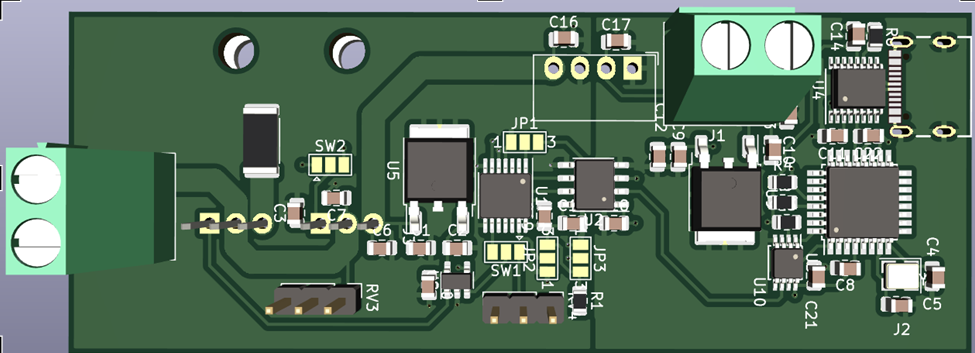
\includegraphics[scale=0.45]{pcb_1st_iteration.png}
        \caption{PCB layout of the 1st iteration of the emulator.}
    \end{figure}


In order to make the first iteration cycle quicker and focus on the modular design 
iteration, the team included a singel cell only in the first PCB. The Fontys laser
printer laboratory was used for the production of the first PCB, however, the via pressing
equipment in the laboratory was incomplete, resulting in a fauty connections. This 
deemed the first PCB unusable, therefore the focus was immediately shifted on the 
second iteration, where the PCB would be ordered and made externally.

\subsection{Testing}
Testing text here.

\section{Second Iteration}
\IEEEPARstart
{T}{he} second iteration of the design\dots

\subsection{Architecture \& Modularity}
Modularity and architecture text here.
    \subsubsection{Model board}
    Model board text here.
    \subsubsection{Cell board}
    Cell board text here.   

\subsection{Software}
Software text here.
\subsection{Current sourcing}
Current sourcing text here.
\subsection{Current sinking}
Current sinking text here.
\subsection{PCB}
PCB text here.
\subsection{Testing}
Testing text here.


\section{Conclusion}
The conclusion goes here.





% if have a single appendix:
%\appendix[Proof of the Zonklar Equations]
% or
%\appendix  % for no appendix heading
% do not use \section anymore after \appendix, only \section*
% is possibly needed

% use appendices with more than one appendix
% then use \section to start each appendix
% you must declare a \section before using any
% \subsection or using \label (\appendices by itself
% starts a section numbered zero.)
%


\appendices
\section{Proof of the First Zonklar Equation}
Appendix one text goes here.

% you can choose not to have a title for an appendix
% if you want by leaving the argument blank
\section{}
Appendix two text goes here.


% use section* for acknowledgment
\section*{Acknowledgment}


The authors would like to thank...


% Can use something like this to put references on a page
% by themselves when using endfloat and the captionsoff option.
\ifCLASSOPTIONcaptionsoff
  \newpage
\fi



% trigger a \newpage just before the given reference
% number - used to balance the columns on the last page
% adjust value as needed - may need to be readjusted if
% the document is modified later
%\IEEEtriggeratref{8}
% The "triggered" command can be changed if desired:
%\IEEEtriggercmd{\enlargethispage{-5in}}

% references section

% can use a bibliography generated by BibTeX as a .bbl file
% BibTeX documentation can be easily obtained at:
% http://mirror.ctan.org/biblio/bibtex/contrib/doc/
% The IEEEtran BibTeX style support page is at:
% http://www.michaelshell.org/tex/ieeetran/bibtex/
%\bibliographystyle{IEEEtran}
% argument is your BibTeX string definitions and bibliography database(s)
%\bibliography{IEEEabrv,../bib/paper}
%
% <OR> manually copy in the resultant .bbl file
% set second argument of \begin to the number of references
% (used to reserve space for the reference number labels box)
\begin{thebibliography}{1}

\bibitem{IEEEhowto:kopka}
H.~Kopka and P.~W. Daly, \emph{A Guide to \LaTeX}, 3rd~ed.\hskip 1em plus
  0.5em minus 0.4em\relax Harlow, England: Addison-Wesley, 1999.

\end{thebibliography}

% biography section
% 
% If you have an EPS/PDF photo (graphicx package needed) extra braces are
% needed around the contents of the optional argument to biography to prevent
% the LaTeX parser from getting confused when it sees the complicated
% \includegraphics command within an optional argument. (You could create
% your own custom macro containing the \includegraphics command to make things
% simpler here.)
%\begin{IEEEbiography}[{\includegraphics[width=1in,height=1.25in,clip,keepaspectratio]{mshell}}]{Michael Shell}
% or if you just want to reserve a space for a photo:

\begin{IEEEbiography}{Youri Tils}
Biography text here.
\end{IEEEbiography}

\begin{IEEEbiography}{Nikola Panchev}
Biography text here.
\end{IEEEbiography}

\begin{IEEEbiography}{Robin van den Dungen}
Biography text here.
\end{IEEEbiography}

\begin{IEEEbiography}{Hein Verhallen}
Biography text here.
\end{IEEEbiography}

\begin{IEEEbiography}{Wyatt Southard}
Biography text here.
\end{IEEEbiography}

% You can push biographies down or up by placing
% a \vfill before or after them. The appropriate
% use of \vfill depends on what kind of text is
% on the last page and whether or not the columns
% are being equalized.

%\vfill

% Can be used to pull up biographies so that the bottom of the last one
% is flush with the other column.
%\enlargethispage{-5in}



% that's all folks
\end{document}